\documentclass{article}
\usepackage[utf8]{inputenc}
\usepackage{amsmath}
\usepackage{graphicx}
\usepackage{hyperref}
\parindent=0pt
\usepackage[a4paper, total={165mm, 235mm}]{geometry}
\usepackage[section]{placeins}
\usepackage{enumitem}
\usepackage{caption}
\usepackage{parskip}
\usepackage{multirow}
\usepackage{biblatex}
\addbibresource{Bibliography.bib}
\usepackage{wrapfig}

\title{PySPI for Persistent Sources}
\author{Möller, Julius}
\date{June 2023}

\begin{document}

\begin{titlepage}
    
    
\includegraphics[height=1cm]{Images/General/MPE_logo_189x180px.jpg}
    \hfill
    
\includegraphics[height=1cm]{Images/General/PH.pdf}
    
\includegraphics[height=1cm]{Images/General/tumlogo.pdf}

    \begin{center}
        \vspace{1cm}
        \large

        Max Planck Institute for Extraterrestrial Physics
        

        \vspace{1.5cm}
        \large
        Thesis for Master of Science in Astrophysics
        
        \vspace{3cm}
        \Huge
        PySpi for Persistent Sources
        
        \vspace{3cm}
        
        \LARGE
        Julius Möller
        
        \vspace{1.5cm}
        \large
        June 2023
        
        
        \vspace{6.5cm}
        
        
        
        \large
        Technische Universität München

        Fakultät für Physik
        
        
        
    \end{center}
\end{titlepage}


\tableofcontents

\pagebreak

\section{About INTEGRAL}




The INTErnational Gamma-Ray Astrophysics Laboratory (INTEGRAL) is an ESA space telescope with contributions from NASA and the RKA. Its mission began on October 17, 2002, when a Proton-DM2 rocket launched it from the Russian Baikonur spaceport in Kazakhstan into a 3-day, highly elliptical orbit with an apogee of 153000km and a perigee of 9000km, although this has not remained constant over the course of its lifetime. This places INTEGRAL mostly above radiation belts that would cause high instrumental backgrounds from charged-particle activation, and is why data collecting is halted during hours of close Earth-proximity. Initially, INTEGRAL had a 2+3-year planned lifetime, which it has greatly exceeded due to its lower than expected fuel consumption. Since then, its science operations have been repeatedly extended, currently up to the end of 2024, with some difficulties along the way such as its failed thrusters in July 2020 (compensated through the use of reaction wheels) and an uncontrolled tumbling caused by a single event upset in September 2021. The satellite is predicted to reenter Earth's atmosphere in 2029.

Onboard INTEGRAL are two main instruments: the Imager on-Board the INTEGRAL Satellite (IBIS) and the SPectrometer of INTEGRAL (SPI). IBIS specializes in being able to locate sources effectively. With an angular resolution of 12 arcmin, it can locate bright sources with arcmin precision in its $9^\circ \times 9^\circ$ field of view, and covers an energy range from 15keV to 10MeV. 

\subsection{About SPI}

\begin{wrapfigure}{r}{0.60\textwidth}
    \begin{center}
      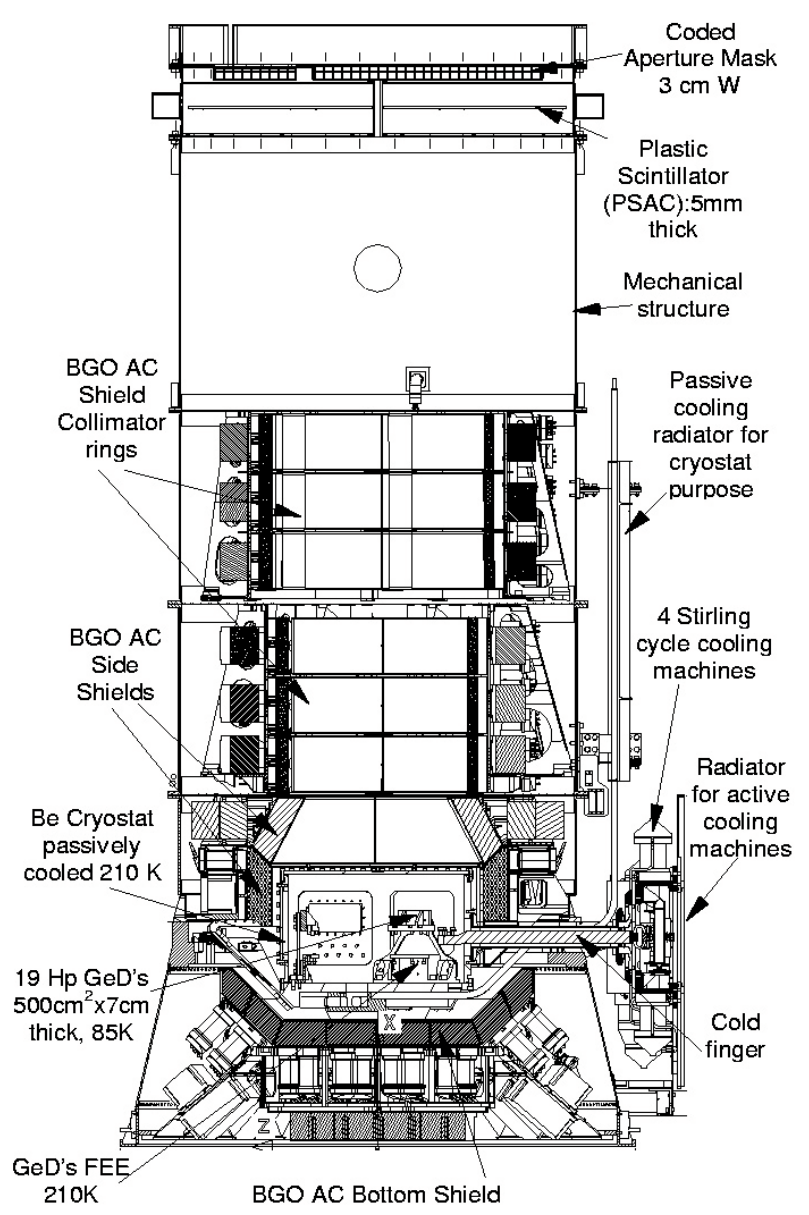
\includegraphics[width=0.58\textwidth]{Images/General/SPI_cut_view_verdenne_2003.PNG}
    \end{center}
    \caption{Cut-out view of the SPI spectrometer \cite{refId0}.}
    \label{SPI cut view}
\end{wrapfigure}




SPI, the instrument used in this Thesis and illustrated in figure \ref{SPI cut view}, specializes in its detailed energy resolution. At 1.3MeV, it is able to resolve energies with 2.5keV precision. It has a field of view of $16^\circ$ and an energy range covering 20keV to 8MeV. One decisive advantage SPI has in comparison to many comparable instruments is that its response matrices are based on extensive ground calibrations and Monte-Carlo simulations, as opposed to relying on astronomical sources such as the Crab Nebula.

\subsubsection*{Detectors}
SPIs detectors are composed of an hexagonal array of 19 reverse-electrode n-type germanium detectors. With a mean crystal weight of 951g and mean volume of $178\text{cm}^3$, the total geometrical area for a flux parallel to the axis is $508\text{cm}^2$. Under normal working conditions, a voltage of 4000V is applied to each detector independently, and this voltage is variable between zero and 5000V. 

The germanium detectors require temperatures below 100K to work effectively, preferably as low as 85K in order to slow the effects of radiation damage. To accomplish this, SPI is equipped with an active cryogenic system. The Ge array is fixed on a Be plate, which is placed inside the cryostat. The plate is connected to the Stirling cycle cryocoolers to provide active cooling. 

Despite the low temperatures and hexagonal design to reduce the probability of hole traps in the semiconductor, radiation damage will inevitably accumulate over the course of a year or more. To combat this issue the detectors can undergo an annealing process, in which they are held at a temperature of $105^\circ \text{C}$ over the course of one or two days, depending on the damage. An annealing process of two days is enough to fully recover the energy resolution after radiation damage leading to a 20\% increase in the FWHM at 1.3MeV \cite{refId0}.

Each detector is connected to a preamplifier, which outputs the charge integrated signal (proportional to the measured energy) and the PSD signal (see below) to the detectors respective electronic chains for processing.

\subsubsection*{Pulse Shape Discrimination electronics (PSD)}
In order to suppress background events, SPI is equipped with Pulse Shape Discrimination (PSD) electronics. The idea is that localized beta decays in the detector material, which would otherwise be indistinguishable from photon energy deposits, only interact in a small volume of the detector, resulting in a single current pulse in the preamplifier. Gamma-rays, which primarily deposit energy via multiple compton scatterings in the detector volume, thus lead to a broader signal. 

Each detector is connected to its own PSD electronic system, which is only triggered in a certain energy range. The lower level threshold (LLD) is configurable, and has been varied between 400keV and 750keV over the missions lifetime, where as the upper level threshold (ULD) is fixed at around 8MeV. Naturally, processing and analyzing the shape of a signal takes time, and when another event is measured within this time it is stored without any PSD information. The PSD electronics thus have an efficiency that can be approximated around 85\% \cite{Roques}.

\subsubsection*{Anticoincidence shield (ACS)}
To further prevent unnecessary background counts in the detectors an anticoincidence shield (ACS) is installed around various of SPIs components (see figure \ref{SPI cut view}). It consists of 91 BGO crystals with a volume of approximately $790\text{cm}^3$ each. Whenever an event is measured simultaneously in the ACS and in the Ge detectors it is vetoed. 

\subsubsection*{Mask}
\begin{wrapfigure}{r}{0.35\textwidth}
    \begin{center}
      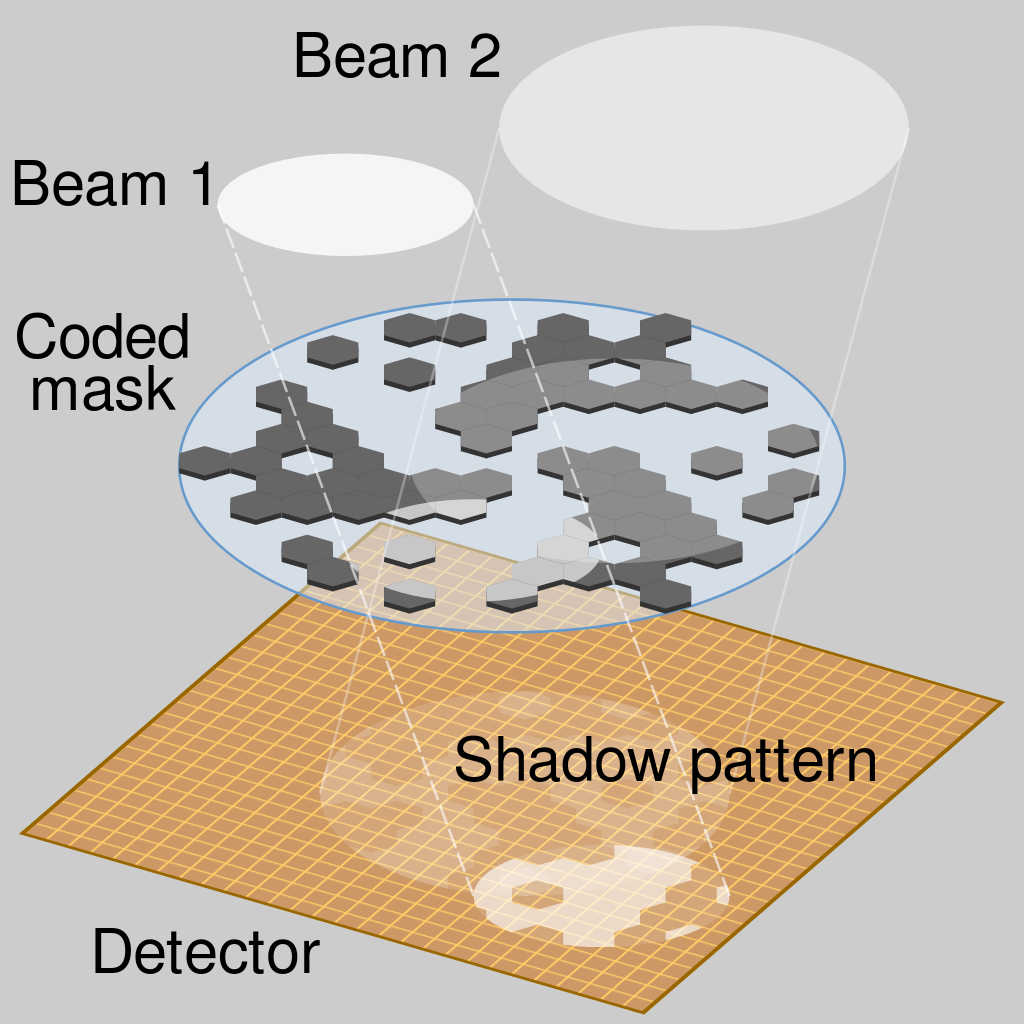
\includegraphics[width=0.33\textwidth]{Images/General/HURA_hexagonal_coded_aperture_mask_principle.svg.png}
    \end{center}
    \caption{The effect of SPIs mask on incoming source beams \cite{HURA}.}
    \label{HURA}
\end{wrapfigure}



Before any photons can reach the array of detectors, they must pass through the coded aperture mask made of a 3cm thick tungsten alloy, located 1.71m above. The $120^\circ$ rotationally symmetric mask is composed of 127 hexagonal tiles (63 opaque and 64 transparent to gamma radiation in the operating energy range) measuring 60mm side to side, and is inscribed within a circle with 720mm diameter. The effect that the mask has on incoming source beams is illustrated in figure \ref{HURA}, and the way this might influence the number of source counts measured in the detector array is visualized for an example source in figures \ref{spegert_pointings_pattern} and \ref{spegert_pointings_pattern_close_up}. This illustrates how we may infer both the source spectrum and position from the detector counts using multiple offset pointings of an astronomical source.

\begin{figure}[h]
  \centering
  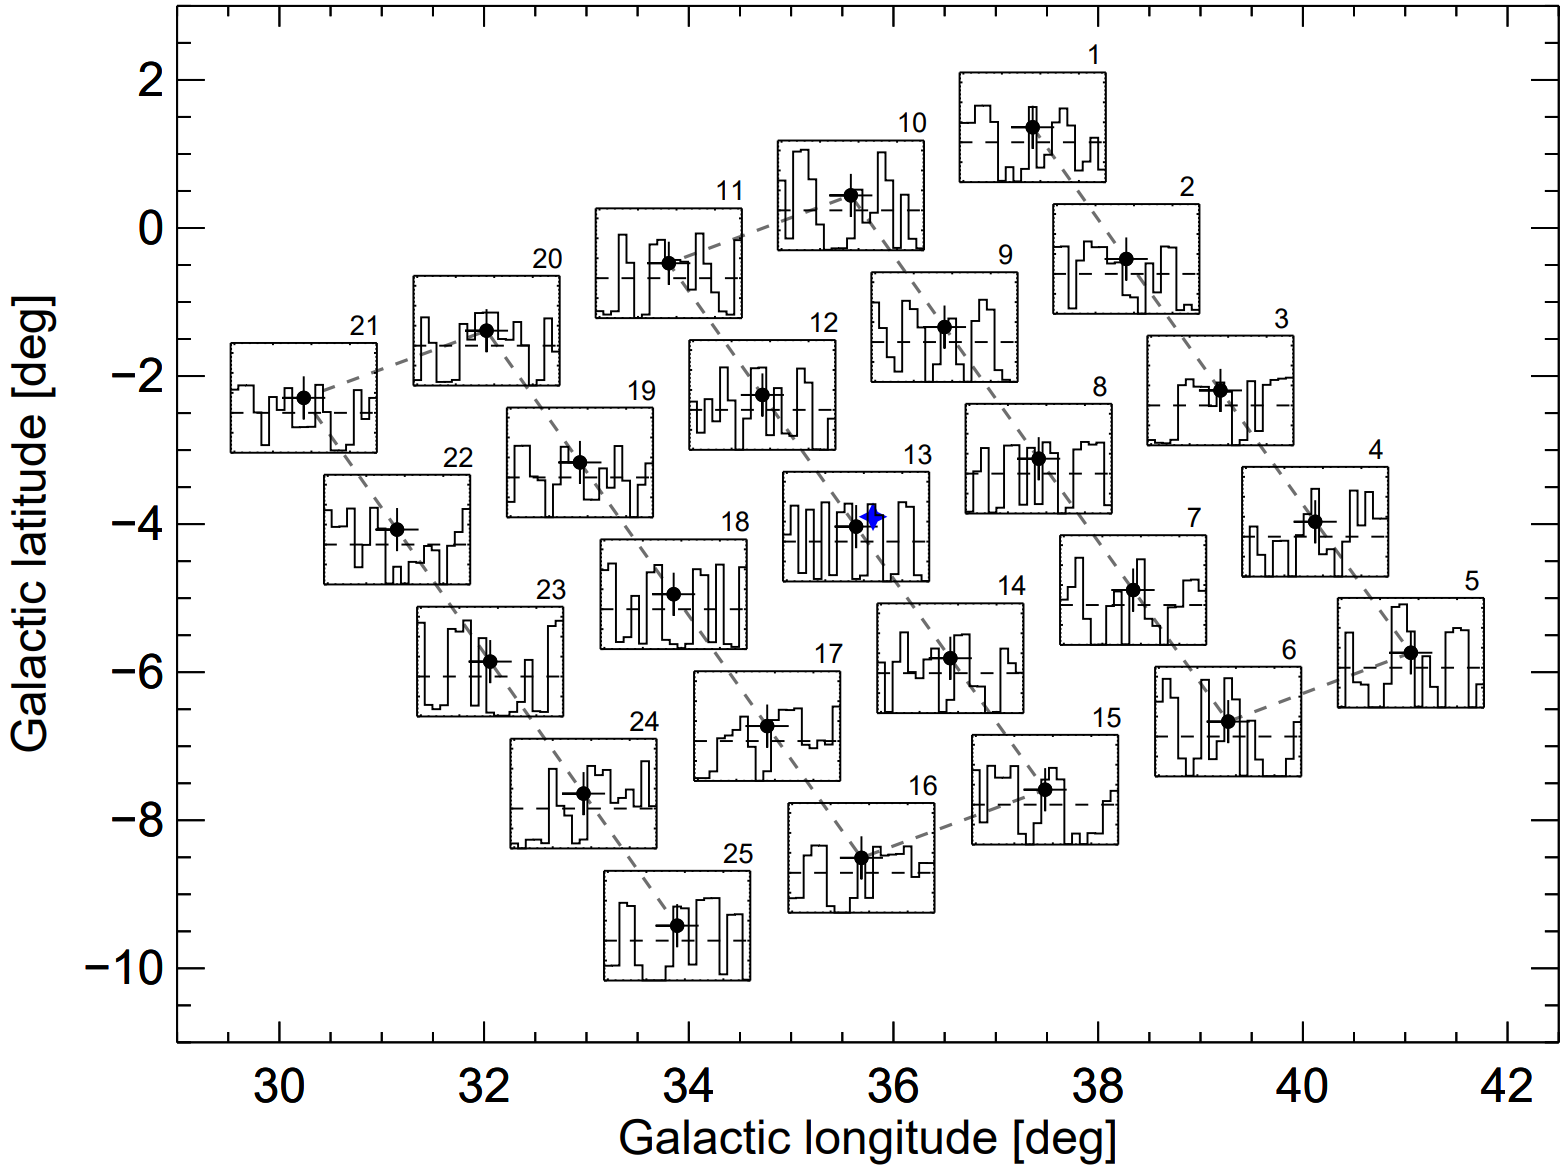
\includegraphics[width=\textwidth]{Images/General/Siegert_PHD_Pointings_pattern.PNG}
  \caption{A typical SPI $5\times5$ grid pointing pattern, each $2.1^\circ$ apart, marked with black dots and sequence number. The blue star in the center represents a celestial source, and the inset panels show the relative detector patterns from the celestial source. A close-up of pointing 13 is shown in figure \ref{spegert_pointings_pattern_close_up}. \cite{dissertation}}
  \label{spegert_pointings_pattern}
\end{figure}

\begin{figure}[h]
  \centering
  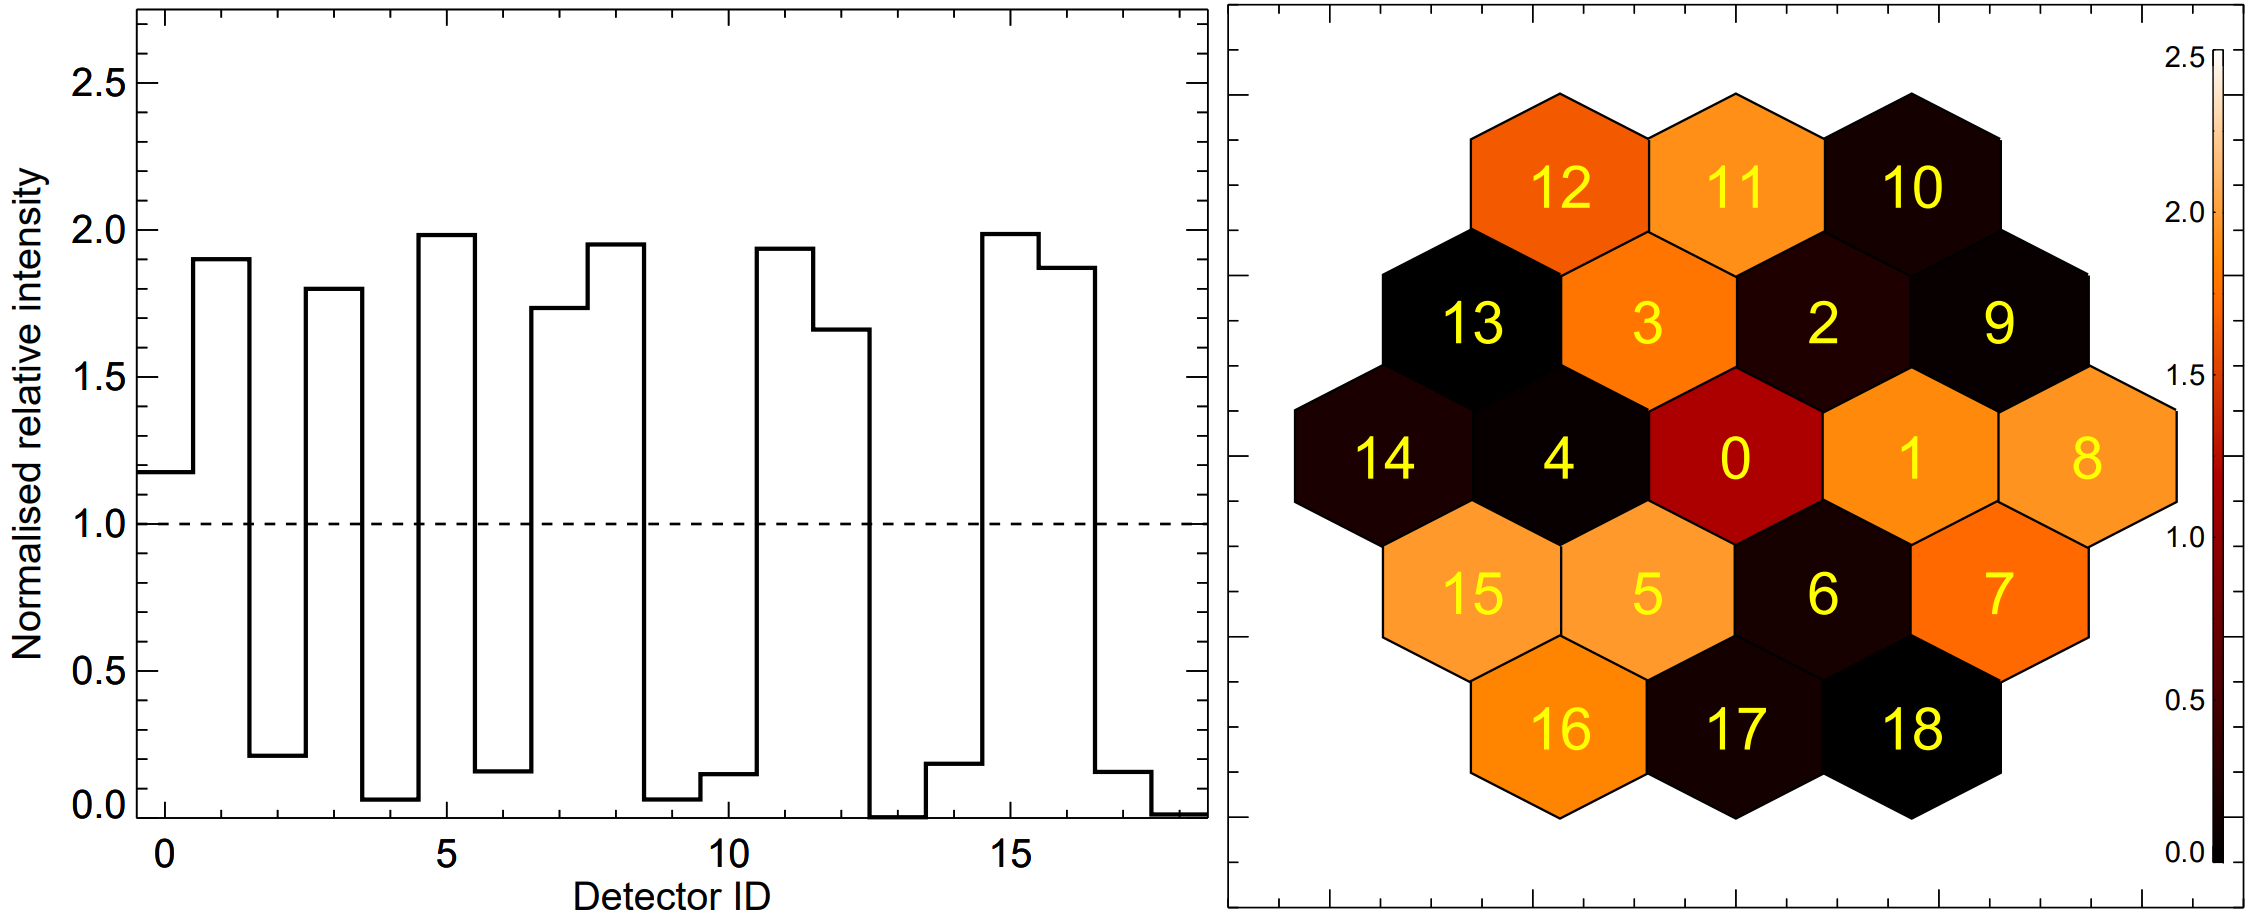
\includegraphics[width=\textwidth]{Images/General/Siegert_PHD_P13.PNG}
  \caption{A close-up of pointing 13 from figure \ref{spegert_pointings_pattern}. On the left we see the relative detector pattern caused by the source in a step plot, and on the right we see the same information displayed as a shadowgram on the detector array. \cite{dissertation}}
  \label{spegert_pointings_pattern_close_up}
\end{figure}

\FloatBarrier

\subsubsection*{Event Types}
\begin{wrapfigure}{r}{0.6\textwidth}
  \begin{center}
    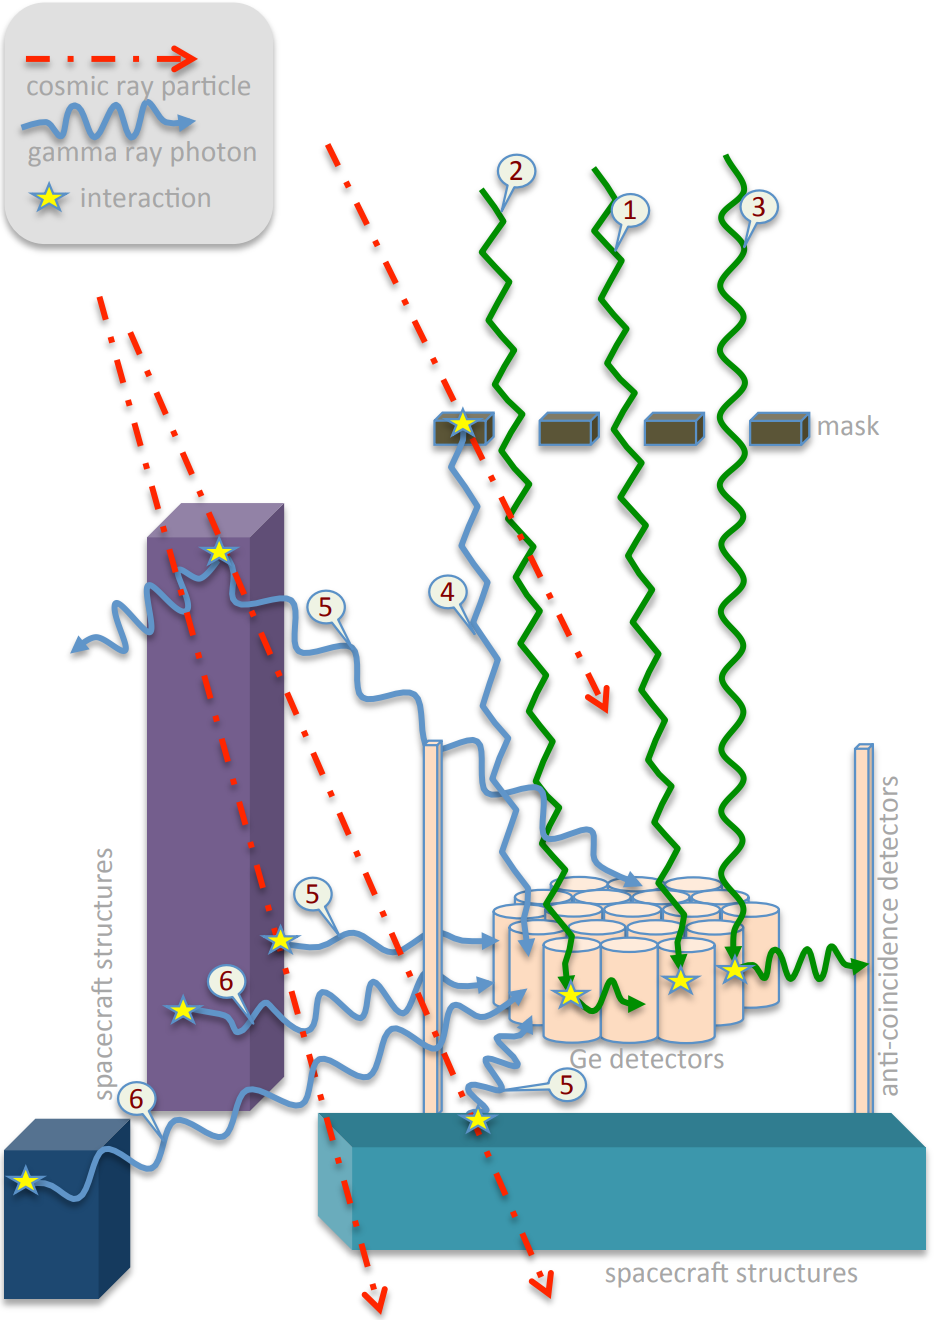
\includegraphics[width=0.58\textwidth]{Images/General/SPI_event_types_roland_2017.PNG}
  \end{center}
  \caption{Illustrations of different event types measured by SPI. Incoming source photons (green) may be absorbed in one detector (1), multiple detectors (2), or be self-vetoed by interacting with the ACS (3). Cosmic particles may interact with surrounding structures, resulting in background photons (blue)(4,5,6). Although the ACS helps suppress these events, they still occur. \cite{refId2}}
  \label{event_types}
\end{wrapfigure}

Figure \ref{event_types} shows some of the different event types measured by SPI. These are generally classified 
se missing due to pe

\subsubsection*{Spurious Events}
spurious events, psd
SE missing from spurious




\pagebreak

\nocite{*}
\printbibliography



\end{document}